\documentclass[12pt]{article}
\usepackage{amsmath,amssymb,amsthm}
\usepackage{graphicx,mathabx}
\usepackage{xcolor}
\usepackage{tikz}
\usepackage{placeins}
\usepackage{lipsum}
\usepackage[shortlabels]{enumitem}
\begin{document}
\title{TCSS 343 - Week 2}
\author{Jake McKenzie}
\maketitle
\noindent\centerline{\textbf{Divide and Conquer}}\\\\\\\\\\\\\\\\
\begin{center}
``If anyone on the verge of action should judge himself according to the outcome, he would never begin." \\$\dots$\\ S$\o$ren Kierkegaard
\end{center}
\begin{center}
    ``A common mistake that people make when trying to design something completely foolproof is to underestimate the ingenuity of complete fools."
\end{center}
\begin{center}
$\cdots$\\
 Douglas Adams
\end{center}
\begin{center}
    ``With your career don't expect anything revolutionary. If you're used to learning it gets easier to learn. Assume walking in that you can learn whatever it is that you need to learn to do the job. If you go to college you should be learning how to learn."\\
    $\cdots$\\
     Paul Sidenblad (Satalite Computer Engineer)
\end{center}

\newpage
\noindent On the previous worksheet I had you write code for binary search. I want you to become more and more comfortable with trees and $\log{n}$ time/space. \\\\
Remember that work is just a function of ``How many problems we have" and ``the amount of work for each problem". Recursion trees is an expressive way of illustrating the ``work" of recurrence problems.\\\\
This will appear to be a digression but they are actually tightly connected ideas. Now remember the geometric series?
$$a + ar + ar^2+ar^3+\dots + ar^{n-1} = a\frac{1-r^n}{1-r}$$
Good, yeah I know who could have forgotten it!? It's one of my favourite series and it should be your best friend right about now.The geomtric series is a series which progresses by some multiplicative factor. \\\\
0. The first thing I will have you do is find $O(a\frac{1-r^{n}}{1-r})$ for two cases. When $r>1$ and $r<1$ where $a$ is some function of $n$.\\\\\\\\\\\\
\newpage
\noindent 1. Now that you've solved for those worst-case runtimes keep them for later because they're going to be useful! Now hold onto your butts because we're going to be having a lot of fun today. Complete this tree given the following recurrence for two more levels(The $a$ need not be the same as the previous $a$...sorry a habit of notation):\\
\centerline{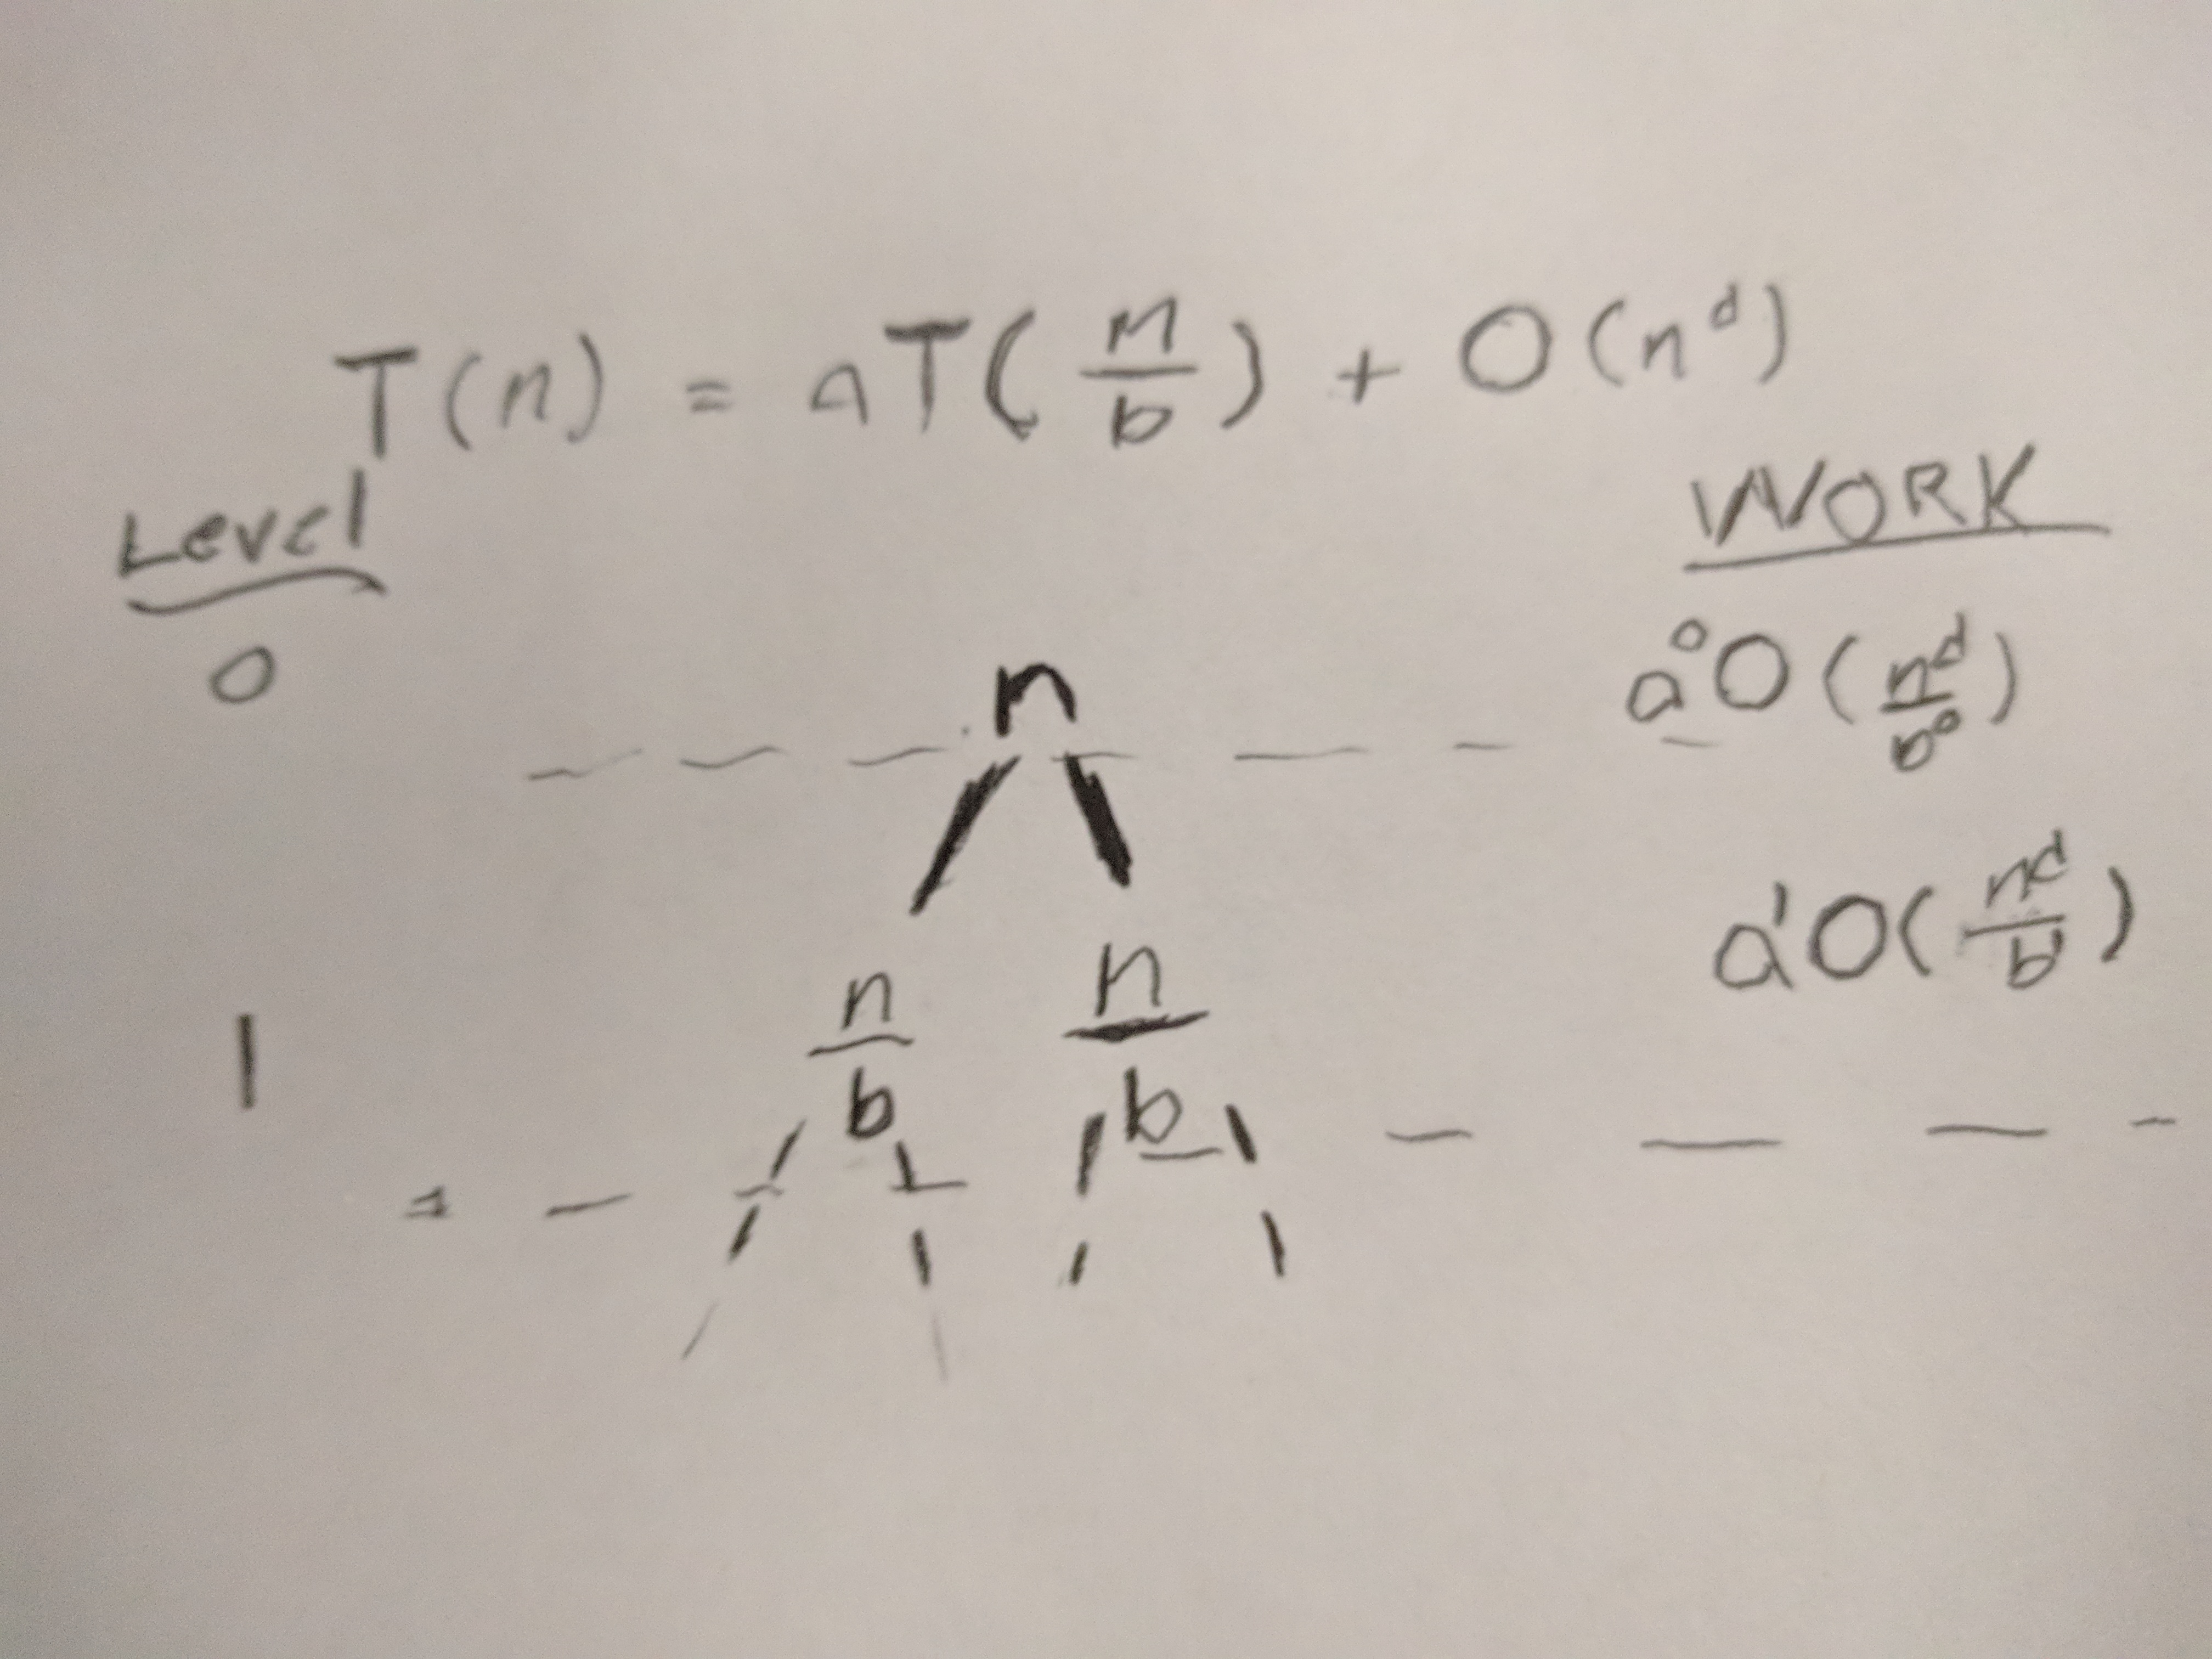
\includegraphics[scale = 0.05]{tree.jpg}} 
\newpage
\noindent 2. Take your previous result, at what level does the tree terminate?\\\\\\\\\\\\\\\\\\\\
3. Please, please try your darndest to express the total work as a summation. Remember: Work is just a function of ``How many problems we have" and ``the amount of work for each problem".
\newpage
\noindent 4. Solve for the three worst cases of the summation you found, when $r<1$, $r=1$ and $r>1$. 
\newpage
\noindent 5. Show that $n^{2.1} \in O(n^2\log{n})$ or that it isn't.\\\\\\\\\\\\
6. The cashier's algorith: \textbf{At each iteration, give the largest coin value $\leq$ the amount to be paid.} A coin system is ``canonical" if the cashier's algorithm returns back the lowest amount of possible counts. Is the common US coin system, $\{25,10,5,1\}$ canonical? How about abount $\{16,9,4,1\}$ or $\{11,7,5,1\}$? What proof technique might you use to prove this? (Please don't move on without giving this some deep justification, it's important. Talk to your peers.) What coins could we add to the US system to make it MORE canonical meaning we can give back even less change than we already do on average?\\\\\\\\\\\\\\\\\\\\\\\\\\
7. Arrange the following in increasing order of asymptotic growth rate.
\begin{enumerate}
    \item[a)]$\frac{n^2}{\log{n}}$
    \item[b)]$\frac{n^2}{2}$
    \item[c)]$2^{3\sqrt{\log{n}}}$
    \item[d)]$n(\log{n})^{1000}$
    \item[e)]$2^{n\log{n}}$
    \item[f)]$2^{\log{n}-\log{\log{n}}}$ 
\end{enumerate}
\newpage
\noindent 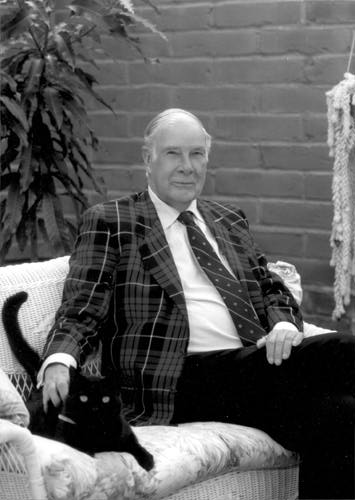
\includegraphics[scale = 0.2]{hamming_cat.jpg}\\
``The purpose of computing is insight, not numbers" - Richard Hamming\\\\
\noindent 8. Alright, alright I know...this isn't a math class this is an algorithms course! But if you solved those problems you now have a wonderful grab bag of results that you can use for now and forever! Now let's do some code.\\\\
Richard Hamming is one of my idols. He was a computer engineer who did a lot of really cool stuff and today we're going to calculate the distance that is named after him!\\\\
The Hamming distance between two integers is the number of positions at which the corresponding bits are different. \textbf{Given two integers $x$ and $y$, can you calculate this distance for me? Well...if not for me at least for Richard's cat.}\\\\
\textbf{Note:}\\
$0 \leq x$,$y < 2^{31}$\\
\textbf{Example:}\\\\
\textbf{Input:} $x = 1$, $y = 4$\\\\
\textbf{Output: } $2$\\\\
\textbf{Explanation: }\\
\noindent 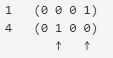
\includegraphics{hamming.jpg}\\
The above arrows point to positions where the corresponding bits are different(next page).\\\\
Write for me (or Richard's cat :3) some code to compute the hamming distance between two integers.
\newpage
9. I'm going to ask you a lot of pop corn questions for now on but that doesn't mean I want you to treat them lightly. This is to test \textbf{YOUR} understanding not the \textbf{INTERNET}. Please do not google the answers. I know you can. I could when I was in this class but please, please don't. Think hard about these now and I'll post the solutions later.\\\\\
\noindent 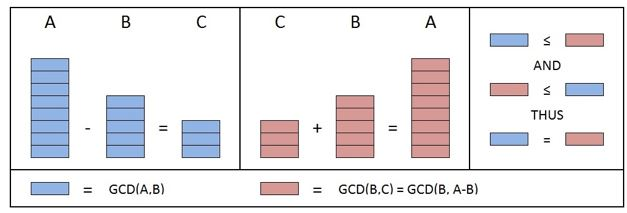
\includegraphics[scale = 0.5]{ea.jpg}
\noindent 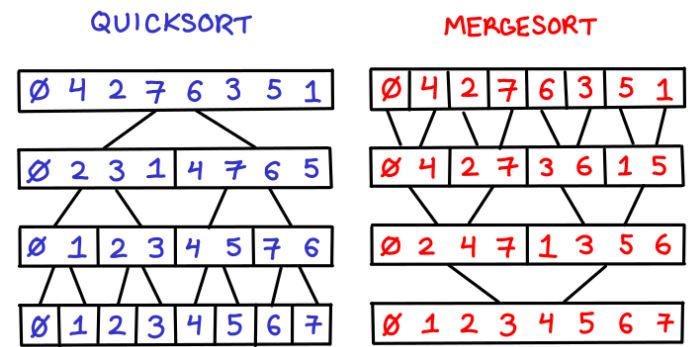
\includegraphics[scale = 0.35]{qsms.jpg}
\noindent 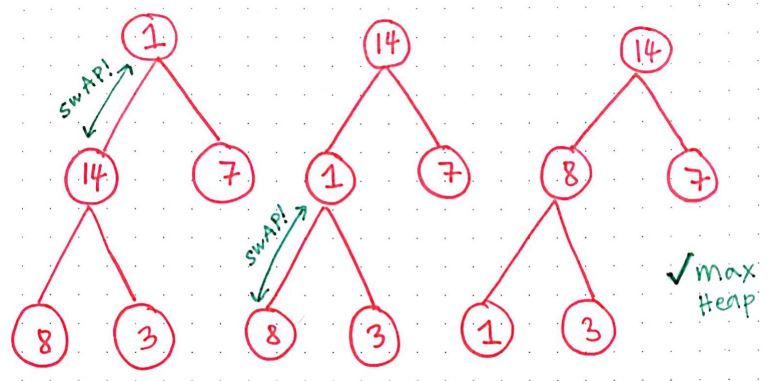
\includegraphics[scale = 0.5]{hs.jpg}\\
Which of the following algorithms is \textbf{NOT} a divide and conquer algorithm by nature?\\
\begin{enumerate}
    \item[a)]Euclidean algorithm to compute the GCD
    \item[b)]Heap Sort
    \item[c)]Merge Sort
    \item[d)]Quick Sort
\end{enumerate}
\newpage
\noindent 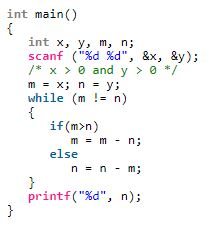
\includegraphics{c.jpg}\\
A. Consider the following c program above, what does it compute?
\begin{enumerate}
    \item[a)]The greatest common divisor of $x$ and $y$
    \item[b)]$x + y$ using repeated subtraction
    \item[c)]$x \mod y$ 
    \item[d)]The least common multiple of $x$ and $y$
\end{enumerate}
B. Maximum Subarray Sum problem is to find the subarray with maximum sum. For example, given an array \{4, -10, 7, 9, -8, -5, 2, 0, -2, 8\}, the maximum subarray sum is 16. The naive solution for this problem is to calculate sum of all subarrays starting with every element and return the maximum of all. We can solve this using Divide and Conquer, what will be the worst case time complexity using Divide and Conquer. Hint: Brute force has $\binom{n}{2}$ total subarrays. Knowing this can you find worst case for brute force?\\
\begin{enumerate}
    \item[a)]$O(n)$
    \item[b)]$O(n\log{n})$
    \item[c)]$O(\log{n})$
    \item[d)]$O(n^2)$
    \item[e)]Not even Jake knows.
\includegraphics[scale = 0.2]{cry.jpg} 
\end{enumerate}
\newpage
\noindent C. For each of the following function indicated how much the function value will change given that it's argument were increased fourfold? (use Stirling's approximation for $n! \sim$ $(\frac{n}{e})^n\sqrt{2\pi n}$. The $\sim$ means formally this: if $f(n) \sim g(n)$ then $\lim\limits_{n\to\infty}{\frac{f(n)}{g(n)}\to1}$)
\begin{enumerate}
    \item[a)]$\log{n}$
    \item[b)]$\sqrt{n}$
    \item[c)]$n\log{n}$
    \item[d)]$n^2$
    \item[e)]$n!$
    \item[f)]$\log{n!}$
\end{enumerate}
`\\\\\\\\\\\\D. Given two integers $x$ and $n$, say we wrote a function to compute $x^n$ using divide and conquer. What is the recurrence relation and worst case runtime of our function?
\begin{enumerate}
    \item[a)]$T(n) = T(n/2) + c$; $T(n) \in O(n\log{n})$
    \item[b)]$T(n) = T(n/2) + n$; $T(n) \in O(n\log{n})$
    \item[c)] $T(n) = 2T(n/2) + c$; $T(n) \in O(\log{n})$
    \item[d)]$T(n) = T(n/2) + c$; $T(n) \in O(\log{n})$
\end{enumerate}
\newpage
\noindent 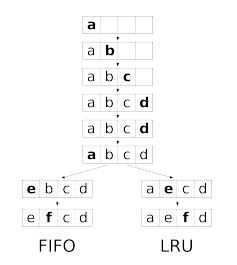
\includegraphics{fifolru.jpg}\\
E. In undergraduate algorithms we typically worry about worst case analysis, but problems can be hard when it doesn't matter. In a computer there is a small speedy memory (the ``cache”) and a big sluggish memory (typically a ``harddisk"). Imagine there are two competing programs, one uses ``Least Recently Used" algorithm and another using ``First In First Out" that periodically issue read and write requests to data stored on ``pages” in the big sluggish memory. If the requested page is also in the cache, then we can happily say it can be accessed directly! If not :( we get what is known as a ``page fault” a.k.a. ``cache miss” — the requested page needs to be brought into the cache, and this requires evicting an incumbent page. The key algorithmic question is then: \textbf{which page should we evicted}? Which algorithm do you think has the worst case runtime and which do you think works better in practice? Why? Is there an intuitive answer to this reality?\\
\begin{enumerate}
    \item[a)]Least Recently Used
    \item[b)]First in First Out
\end{enumerate}
\newpage
\noindent F. Given two sorted arrays of n distinct integers Y[$1,\dots,n$] and Z[$1,\dots,n$]. Supposed that Y[$1,\dots,n$] is arranged in decreasing order and Z[$1,\dots,n$] is arranged in increasing order.
You want to find out whether there is an index i for which Y[i] = Z[i]. Give an algorithm that runs in time $O(\log{n})$ for this problem. Hint: given that you know the runtime is $O(\log{n})$ can you use the recurrence relation to work backward to find what the algorithm should be?
\newpage
\noindent 11. Any comparison based sorting algorithm must make at least f(n) comparisons. Show that is f(n) $\in \Omega(n\log{n})$. Hint: How many possible ways are there are there of choosing, without replacement $n$ things from $n$ where order matters.
\begin{enumerate}
    \item[a)]$\log{n!}$
    \item[b)]$n^2\log{n}$
    \item[c)]$\log{n}$
    \item[d)]$n$
\end{enumerate}
12. At what step does the divide and conquer strategy run into problems?
\begin{enumerate}
    \item[a)]Divide step.
    \item[b)]Conquer step.
    \item[c)]Recombine step.
\end{enumerate}
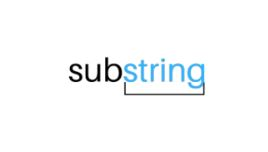
\includegraphics[scale = 0.75]{substring.jpg}\\
13. Say I give you the string ``substring" and want you to return back ``string", what did I ask you to return?
\begin{enumerate}
    \item[a)]Coda
    \item[b)]Tail
    \item[c)]Prefix
    \item[d)]Suffix
\end{enumerate}
\end{document}